\section{SAT Encoding}
\subsection{Concept}
The concept of SAT, also known as the Boolean Satisfiability problem,
is a computer science problem aimed at determining the satisfiability of a propositional logic formula.

\begin{flushleft}
    \textbf{Input}: A propositional logic formula, typically represented in Conjunctive Normal Form\cite{cnf} (CNF).
\end{flushleft}

\begin{flushleft}
    \textbf{Output}:
\end{flushleft}
\begin{itemize}
    \item SAT (Satisfiable): If there exists a truth value assignment (true/false) to the
          logical variables that makes the original propositional logic formula evaluate to true.
    \item UNSAT (Unsatisfiable): If every truth value assignment (true/false) to the
          logical variables results in the original propositional logic formula evaluating to false.
\end{itemize}

\subsection{Encoding}
SAT Encoding is a method in which certain problems can be solved by transforming
them into SAT problems: representing problems using propositional logic formulas and
applying SAT Solvers to solve these propositional logic formulas\cite{pham_ngoc_anh}.

\begin{figure}
    \centering
    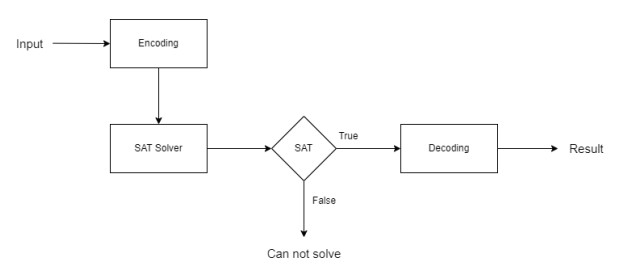
\includegraphics[width=0.9\textwidth]{chapter1/image/flow_sat.jpg}
    \caption{SAT Encoding Process}
    \label{fig:sat_encoding_process}
\end{figure}

A problem solved using SAT Encoding follows the following steps: First, identify the
input data or the problem's input that needs to be solved. The Encoding module then
takes this input data, defines the rules, and encodes these rules into Conjunctive Normal
Form\cite{cnf} (CNF) logical formulas, producing an output file containing the number of
variables, the number of clauses, and the CNF formulas. The SAT Solver takes the
output file from the Encoding module as input, processes the expressions, and generates
the output result. The output result can be SAT if the SAT Solver finds a dataset
satisfying the CNF formulas, or UNSAT if it fails to find any dataset. If the result is
SAT, the SAT Solver provides another file containing the corresponding dataset it
found. From the discovered dataset, the solution to the problem can be inferred, resulting
in the corresponding answer for the input data.

\subsection{SAT Solvers}
SAT Solver is a tool designed to solve the Boolean Satisfiability (SAT) problem,
determining whether a propositional logic formula is satisfiable or not. It utilizes CNF
(Conjunctive Normal Form\cite{cnf}) formulas.

In the SAT problem, we are given n Boolean variables and m clauses, where each clause
is the disjunction of a set of literals, and a literal is a variable or its negation. The aim is
to decide whether there is an interpretation of the variables that satisfies all clauses.
Currently, numerous SAT- tools can efficiently handle a large number of clauses and
variables, providing optimal results. Examples include Minisat\cite{minisat}, Lingeling\cite{lingeling},
Glucose\cite{glucose}, RSat\cite{rsat}.

SAT is proven to be NP-complete\cite{SATNPComplete}, meaning it has exponential time complexity in the
worst case scenario. Despite this, effective and scalable algorithms for SAT have been
developed in the 2000s, significantly advancing the automatic resolution of problems
with tens of thousands of variables and millions of clauses [6]. One such algorithm used
by SAT Solvers is DPLL (Davis-Putnam-Logemann-Loveland), introduced in 1961,
relying on a backtracking, exhaustive search approach.

Modern SAT-solving methods introduced in the 2000s have incorporated the Conflict
Driven Clause Learning (CDCL) algorithm alongside DPLL, enhancing the efficiency
of SAT Solvers in various domains.

Kissat\cite{kissat_jku} is a "keep it simple and clean bare metal SAT solver" written in C.
It is a port of CaDiCaL back to C with improved data structures, better scheduling of inprocessing and optimized algorithms and implementation.
The CNF file format used by Kissat consists of the following components:

\begin{itemize}
    \item The first line specifies the number of variables and the number of clauses in the CNF file.
    \item The subsequent lines contain the CNF-formatted logical statements, represented as clauses.
\end{itemize}

\begin{center}
    \begin{verbatim}
        p cnf [number of variables] [number of clauses]
        [clauses]
    \end{verbatim}
\end{center}

\begin{flushleft}
    In this format:
\end{flushleft}
\begin{itemize}
    \item \texttt{p cnf} denotes the CNF format.
    \item \texttt{[number of variables]} denotes the count of logical variables used.
    \item \texttt{[number of clauses]} represents the number of logical clauses.
    \item \texttt{[clauses]} refers to the CNF-formatted logical statements.
\end{itemize}

For example:
\begin{center}
    \begin{verbatim}
        p cnf 3 2
        1 -2 0
        2 3 -1 0
    \end{verbatim}
\end{center}

This CNF file contains 3 variables and 2 clauses.
The first clause is \texttt{[1 -2 0]}, and the second clause is \texttt{[2 3 -1 0]}.
The \texttt{0} at the end of each clause denotes the end of the clause.
It represented as logical formulas:
\begin{center}
    $(x_1 \vee \neg x_2) \wedge (x_2 \vee x_3 \vee \neg x_1)$.
\end{center}

The SAT problem can be solved by running the Kissat SAT Solver on the CNF file.
The output will indicate whether the logical formula is satisfiable or unsatisfiable
and provide the truth value assignments for the logical variables with format:
\begin{center}
    \begin{verbatim}
        s [status]
        v [variable assignments]
    \end{verbatim}
\end{center}

For this given CNF file, the output will be:
\begin{center}
    \begin{verbatim}
        s SAT
        v 1 -2 -3
    \end{verbatim}
\end{center}

But it is only one of the possible solutions, there are many other solutions that satisfy the CNF formula.
To find all solutions, we need to append the solution found as a clause and run the SAT Solver again.
This process is repeated until the SAT Solver returns UNSAT, indicating that all solutions have been found.

\subsection{Applications}
In addition to SAT Encoding, SAT is utilized in various fields of information
technology. Notable areas include: In formal methods, SAT is used for hardware model
testing, software model testing, and test pattern generation. In the field of artificial
intelligence, SAT is employed for planning, knowledge representation problems, and in
intelligent games. In the realm of automated design, SAT is applied for equivalence
checking, delay computation, error detection, and more.